\documentclass[letterpaper,twocolumn,10pt]{ilass}
\def\thepage{}

%\usepackage{times}
\usepackage{amssymb}
\usepackage{amsmath}
\usepackage{tikz}
\usepackage{graphicx}
\usepackage{gensymb}

\usepackage{graphicx}

\evensidemargin = 0.0in
\headheight = 0.0in
\headsep = 0.0in
\parskip = 0.0in
\parindent = 0.25in
\topmargin    0.00in
\oddsidemargin 0.00in
\textheight    9.00in
\textwidth     6.50in
\columnsep     0.25in

\title{\vspace{-0.25in}
      {\small \em
       ILASS-Americas 29th Annual Conference on Liquid Atomization and Spray Systems,
       Atlanta, GA, May 2017} \newline\newline
      {\large\bf In-Nozzle Flow Investigations of Marine Diesel Injectors} }
				
\author{\large
        R. Balz\textsuperscript{1,2}\footnote{reto.balz@wingd.com},
				A. Schmid\textsuperscript{1},
				D. Sedarsky\textsuperscript{2}\\
				%
				\textsuperscript{1}Winterthur Gas \& Diesel Ltd.,
				Winterthur,	Switzerland\\
				%
				\textsuperscript{2}Chalmers University of Technology,
				Combustion Division, Gothenburg, Sweden}

\date{\normalsize  \centerline{\bf Abstract} \vspace{0.05in}
\begin{minipage}{6.5in} \normalsize
Injector geometries of large marine two-stroke diesel engines differ extensively from
configurations typically used in diesel engines for automotive applications.
In marine engines, the fuel enters the combustion volume radially, supplied by a
multi-hole injector with asymmetrically positioned orifices facing in similar directions
(shallow umbrella angle). Due to this setup, the nominal direction of the orifice group
is also eccentric with respect to the central axis of the injector.
%
Experiments have shown that the sprays formed by this arrangement are asymmetric
with respect to the axis at each orifice. These strong deviations can lead
to wall wetting which increases fuel consumption, emissions, component temperatures and
contributes to loss of lubrication at the wall.
In order to investigate the in-nozzle flow and how it affects the spray morphology in this
design, experiments were carried out using transparent nozzles at injection pressures and
air densities of up to 80~MPa and 35~kg/m$^3$, respectively.
The experiments were performed with diesel fuel in a newly built ambient temperature
spray chamber which was designed to cope with significant spray backsplash.
The results discussed here were generated using an orthogonally arranged 0.75~mm diameter
mono-hole injector which matches the hole size and geometry used in large marine two-stroke
diesel engines.
%
High-speed shadowgraphy using a far-field microscope was applied to visualize cavitation
within the nozzle during the complete injection process. These imaging results are use to
compute statistical evaluations of cavitation in the nozzle over a range of conditions.
\end{minipage} \vspace{-0.25in}}
\baselineskip = 2.0\baselineskip

\begin{document}

\ifpdf
\DeclareGraphicsExtensions{.pdf, .jpg}
\else
\DeclareGraphicsExtensions{.eps, .jpg}
\fi

\maketitle

\clearpage

\pagenumbering{arabic}
\setcounter{page}{2}


%INTRODUCTION
%   --worldwide shipping depends heavily on marine diesel engines
%   --marine diesels high thermal efficiency drives design
%   --emissions are increasingly important
\section*{Introduction}
Maritime shipping currently represents the largest mode of supply for moving goods around
world. Sea transport of goods accounts for more than 53 percent of U.S. imports and 38 percent
of exports (by value)\cite{Blank2012}. The efficiency and prevalence of this transport network
is due in large part to the advantages of large two-stroke marine diesel engines which have
been designed to operate using a variety of highly variable, low cost liquid fuels. 
%
Much of the ongoing marine engine development is focused on meeting the requirements of the
IMO (organisation maritime internationale) Tier III legislation which calls for an 80\%
reduction in $NO\textsubscript{x}$ engine out levels and places more stringent limits on
the fuels which can be used can be used near populated coastlines.

The realization of strategies for reducing $NO\textsubscript{x}$ production by
modifying the in-cylinder combustion, e.g. water in fuel emulsion or dual fuel reaction control,
requires a solid understanding of spray development and mixing during fuel injection.
%
Past experimental work conducted at Winterthur Gas \& Diesel Ltd.~(Win~G\&D) using a
constant volume spray combustion chamber (SCC) with dimensions representative of
smaller two-stroke marine engines (\o 500 x 150~mm) highlights some of the issues
associated with fuel injection for large engines\cite{Herrmann2011}.
Investigations on the SCC have shown that the eccentric and offset nozzle designs utilized
in two-stroke marine engines exhibit spray deflections on the order of
10$^{\circ}$ or more\cite{Schmid2013}.
%
In addition, preliminary work using CFD simulations with an advanced cavitation model
indicates that the two-phase, highly compressible flow inside the nozzle may strongly
influence the spray propagation\cite{Schmid2014}.
%

%   --Cavitation number should be introduced here. Explain what it means and why it's useful.
%   --No need to explain the other definitions used for CN, just be clear about
%     the definition that you are using.
%   --Put in an equation for CN ... refer to it in the text.

%%--cavitation number stuff, moved from 'Results' section.
%Literature uses different non-dimensional cavitation numbers ($CN$) to represent cavitation
%conditions in nozzles. These numbers are usually defined as ratios from pressure in front and
%behind the orifice and the vapour pressure of the liquid \cite{Hult2016, Giannadakis2008}.
%A commonly used one is
%$(p\textsubscript{i} - p\textsubscript{b})/(p\textsubscript{b}-p\textsubscript{v})$,
%where $p\textsubscript{i}$ is the pressure upstream and $p\textsubscript{b}$ the pressure
%downstream the orifice (also called back pressure). $p\textsubscript{v}$ is the vapor pressure
%of diesel and neglected as insignificant for $CN$ when using rail pressures orders of magnitude
%higher.\\
%%

Cavitation often occurs as ``geometric cavitation'', caused by the sudden reduction of
static pressure in the fluid near the corner and wall of the nozzle hole as the flow
enters the passages; or as "string cavitation", appearing transiently near the center of
strong vortices in the flow\cite{Andriotis2008}.
%
Results from Schmid et al. indicate that both of these cavitation forms are important to the
internal flow of injectors designed for use in large two-stroke marine diesel engines.
However, it is not clear how switching from one type of internal flow to another will affect
spray formation and thus spray breakup, fuel mixing, and combustion in a real marine engine
during one cycle.\\
%
These internal flows and their effects with regard to primary breakup currently
strain the capabilities of CFD simulation efforts, and models suitable for optimizing
fuel mixing in large marine diesel engines have yet to be developed. 
%
This is not surprising, since primary breakup is often described as the least understood part of the combustion process \cite{Fansler2015,Linne2013}.

%
In-nozzle flow is a topic of considerable interest, and a variety detailed work using transparent nozzles to study flows related to fuel injection have been presented recently
\cite{Fansler2015, Blessing2003, Duke2014}.
However, this work is most relevant to the injection strategies used in automotive applications.
Hult, et al.\cite{Hult2016} provided visualizations for hole sizes and flow rates related to marine diesel engines, but at fuel pressures limited to around 10~MPa.

Recent efforts at Chalmers University have led to the development of optically
transmissive injector inserts, which can be designed to duplicate production nozzle geometries
and withstand higher fuel pressures than former designs \cite{Falgout2015}.
In this work we combine an adapted Win~G\&D nozzle geometry and a braced insert based on
the Chalmers transparent nozzle design to study internal nozzle flow under engine-like
conditions. This setup enables measurements which can lend insight for model development
and be used in validation of cavitation modeling results for marine engines.
%
Here, we utilize full-scale nozzle geometries, injection pressures, and engine-like
back-pressure conditions designed to match setpoints for Win~G\&D marine diesel engines. 

%NEW SPRAY CHAMBER
%   --add details: what flowrate? how much higher?
\section*{Ambient temperature spray chamber}
Most spray chambers designed for measurements on automotive sprays are not well-suited for
marine engine spray investigations.
Typical nozzle dimensions for large two-stroke diesel engines often involve orifice diameters in the millimeter range.
%

A custom spray chamber was designed and constructed to deal with the rebounding fuel spray.
For the sprays in this work, this rebound is an important design consideration, since the nozzle dimensions, and by extension the fuel flow, are substantially higher than flows typical in small engines. 

\begin{figure}[h]
\begin{center}
\begin{tikzpicture}
\node[inner sep=0pt] (russell) at (0,0){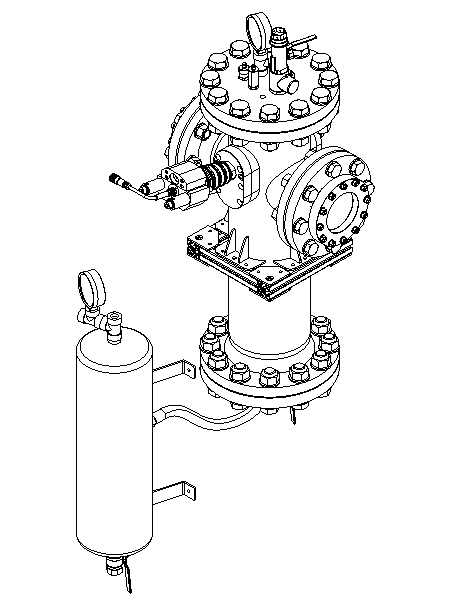
\includegraphics[width=3in]{mark7_ill_iso_1}};
\draw (-0.94in,1.34in) node[]{a};
\draw[dashed] (-0.89in,1.31in) -- (-0.42in,0.87in);
\draw (-0.54in,0.24in) node[]{b};
\draw[dashed] (0.03in,0.05in) -- (-0.49in,0.21in);
\draw (-1.33in,0.19in) node[]{c};
\draw[dashed] (-0.98in,-0.3in) -- (-1.3in,0.16in);
\draw (0.20in,-1.01in) node[]{d};
\draw[dashed] (0.01in,-0.86in) -- (0.16in,-0.99in);
\draw (-0.17in,-1.82in) node[]{e};
\draw[dashed] (-0.64in,-1.79in) -- (-0.22in,-1.82in);
\draw (1.23in,0.40in) node[]{f};
\draw[dashed] (0.76in,0.59in) -- (1.19in,0.4in);
\draw (1.09in,1.69in) node[]{g};
\draw[dashed] (0.42in,1.56in) -- (1.06in,1.7in);
\end{tikzpicture}
\end{center} 
\vspace*{-5mm}
\caption{Isometric view schemata of new spray chamber:
         a) Win~G\&D injector,
				 b) spray chamber,
				 c) auxilliary tank,
				 d) connection hose,
				 e) drainage valve,
				 f) fused silica window,
				 g) safety relief valve and accessories.}
\label{fig1} 
\end{figure}


%
The design of the newly built spray chamber at Chalmers is based on standardized stainless
steel flanges (EN 1092-1) that are welded to a main body formed by a section of
stainless steel pipe with an inner diameter of approximately 200~mm.
%
The use of standard flanges allows a measure of design versatility and reduces the amount of custom machining required to implement the system.
A schematic of the spray chamber is depicted in figure \ref{fig1}.
%
The spray chamber is designed to operate at ambient temperature, primarily in conjunction
with transparent nozzles for coupled measurements of internal flow and the near-nozzle
spray formation region.
%
The transparent nozzle inserts used in the current work are made of PMMA (polymethylacrylate), a thermoplastic with a melting point around 140 to 160$^{\circ}$C.
%
A major objective of the system is to allow observation of the in-nozzle flow and how it
influences the primary breakup of a non-reacting spray. From this standpoint, it is reasonable
that the density and motion of the environment surrounding and interacting with the jet
dominates the breakup behavior, especially near the orifice, and temperature effects can largely be neglected.
%
Incidentally, the flange design of the new chamber was chosen to match the specifications
used in the high-pressure, high-temperature spray chamber at Chalmers. This allows for
testing at high temperatures (up to 900~K) or even higher pressures (up to 100 bar)
without substantial redesign of the experiment if the necessary.
%
The new spray chamber can be filled with nitrogen or air to pressures up to 3~MPa to
match engine-like air densities at ambient temperatures which are around 35~kg/m$^3$.
The main chamber is coupled to a secondary pressure vessel that enables rapid flushing
of the main chamber (see figure \ref{fig1}).
This feature is necessary to reduce rebound and deal with the large amount of fuel
injected into the main chamber, and also prevents window fouling by reducing the number of fine fuel droplets present in the system.
The secondary tank is mounted at a lower position as shown in figure \ref{fig1},
allowing gravity flow collection and disposal residual fuel as well.
A pneumatically driven angle valve is used to control the flushing action of the chamber.
This valve is mounted near the bottom flange of the spray chamber and not visible in figure \ref{fig1}. 

\begin{figure}[h]
\begin{center}
\begin{tikzpicture}
\node[inner sep=0pt] (russell) at (0,0){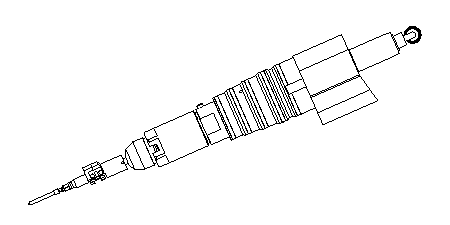
\includegraphics[width=3in]{injector_ill_1}};
\draw (0.21in,0.75in) node[]{a};
\draw[dashed] (0.16in,0.23in) -- (0.2in,0.7in);
\draw (-0.75in,0.3in) node[]{b};
\draw[dashed] (-0.78in,-0.32in) -- (-0.75in,0.25in);
\draw (-1.32in,0.05in) node[]{c};
\draw[dashed] (-1.05in,-0.475in) -- (-1.3in,0in);
\end{tikzpicture}
\end{center}
\vspace*{-5mm}
\caption{Schemata of injector setup:
         a) Win~G\&D injector,
				 b) transparent nozzle holder,
				 c) Kistler pressure sensor.}
\label{fig2} 
\end{figure}

The chamber hardware and controls form a mobile rig that can be moved to accommodate
different experiments.
%
The spray chamber is mounted on a rigid frame, with the control and sensor wiring collected
in an enclosure to simplify and organize connection to the data acquisition hardware.
Pressure and temperature sensors are installed to control the desired air density conditions
within the spray chamber and control the filling and flushing procedures.
%

Line-of-sight optical access through the center of the main chamber is provided by a pair
of windows with optically usable diameters of 120~mm. These optical quality fused silica windows are clamped to the flange surfaces as depicted in figure \ref{fig1}.
The two remaining flanges that are arranged orthogonally with respect to the primary
optical access are configured as dummy (blocked) and for mounting the injector, respectively.
%
The injector mount can be configured to allow a modest angle adjustment to further reduce
rebound from the spray by controlling the impingement angle of the spray plume and
the chamber wall.
%

Original marine diesel injector hardware was provided by Win~G\&D for this work.
This nozzle was subsequently adapted and fitted to a transparent nozzle insert holder
(see figure \ref{fig2}).
To cope with the need for high diesel mass flows for the marine injectors,
a piston accumulator with a total volume of 5~dm$^3$ was used to stabilize
the injection pressure for the duration the injection event (approximately 8~ms). 


%EXPERIMENT
\section*{Experimental setup}
Focused shadow images of the diesel fuel flow inside the transparent nozzle
were acquired over a series of cavitation numbers by varying
the back-pressure maintained by the spray chamber for a given injection pressure
setting.
%
Here, the refractive index of the nozzle material closely matches the index of the fuel such that undisturbed liquid in the channel transmits light with minimal refraction.
When cavitation occurs it produces an immediate and large step in the refractive index
as the fluid phase, pressure, and temperature vary. This index difference refracts source
light causing a dark signature which indicates cavitation in the flow.  
%
Source light in the experiments was supplied by a pulsed diode laser (Cavilux Smart, Cavitar)
operating at 640~nm and set to deliver XX ns pulses at a repetition rate of 20~kHz.
%
The nozzle flow was imaged by a long distance microscope (QM100, Questar)
and acquired by a high-speed CMOS camera (Phantom V1210, Vision Research).
%
The resulting (512~x~800~pixel) digital images were recorded at a framerate of 20,000~fps,
where each image corresponds to a field of view of 2.5 x 3.9~mm (see figure \ref{fig3}). 
%

\begin{figure}[h]
\begin{center}
\begin{tikzpicture}
\node[inner sep=0pt] (russell) at (0,0){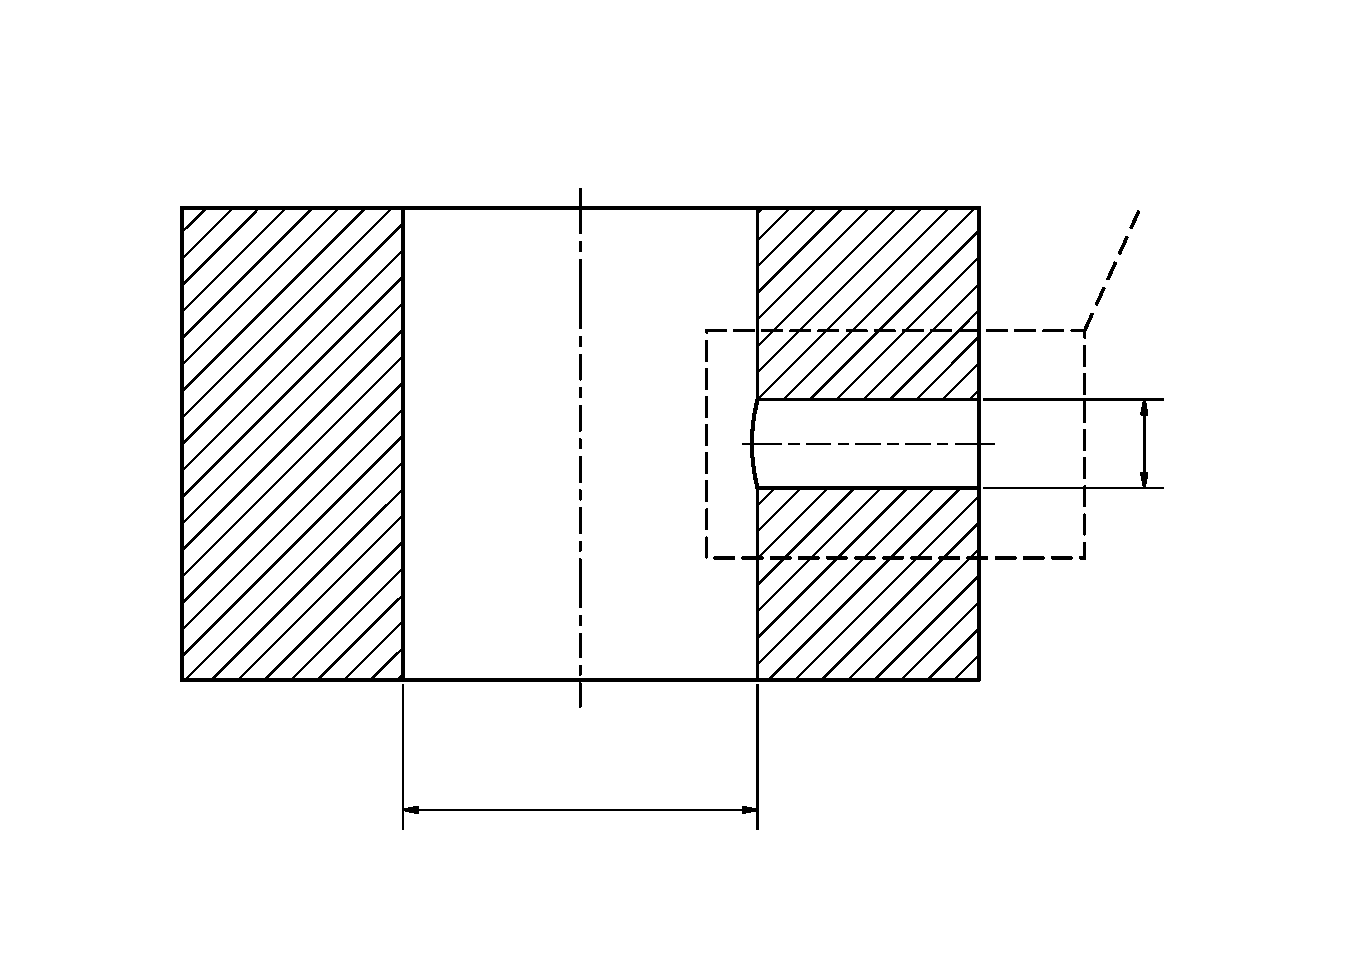
\includegraphics[width=3in]{nozzle_ill}};
\draw (0.98in,0.07in) node[rotate=90]{\o a};
\draw (-0.21in,-0.67in) node[]{\o b};
\draw (1.03in,0.67in) node[]{FOV};
\end{tikzpicture}
\end{center}
\vspace*{-10mm}
\caption{Section view of transparent nozzle made of PMMA with orifice diameter
         \o a = 0.75~mm and sac diameter \o b = 3~mm. The field of view (FOV)
				 of the optical setup used is illustrated as dashed rectangle.}
\label{fig3} 
\end{figure}

National Instruments data acquisition hardware and a LabView interface were set up to run
the spray chamber and compile time-resolved sensor data for the system during the experiments.
%
A Kistler piezo-resistive pressure sensor with a natural frequency over 200~kHz was used
together with a National Instruments USB-6351 DAQ with 1.25~MS/s to measure the fuel pressure
close to the transparent nozzle. The location of the pressure sensor is shown in figure
\ref{fig2} c).
Here the proximity of the sensor to the nozzle allows for accurate measurements as
fuel injectors usually have high pressure loss. Accurate pressure information close to the
orifice is important for understanding boundary conditions.
%

The transparent nozzle section used in the imaging, as shown in figure \ref{fig3},
follows the design developed at Chalmers for studying internal nozzle flow at elevated
pressures\cite{Falgout2016}.
%
% -- Don't try to explain your overall project, since that is generally
%    of less interest to people at the conference, and hard to do well
%    in this limited space. Try to focus on results and what is being done
%    right now as much as possible.
In these initial investigations, the nozzle design is set up to coincide with the
simple the geometry used in the preliminary CFD simulations carried out at Win~G\&D.
%
Here, the nozzle is a basic plain circular orifice, with sharp edges and no taper.
The diameter of the sac volume is 3~mm (see figure \ref{fig3},  {\o b}) and the orifice has a diameter of 0.75~mm (see figure \ref{fig3},  {\o a}) and a length of 1.875~mm.
%
PMMA is used as transparent nozzle material as it has a very similar refractive index as
diesel fuel. This index matching allows visualization of the in-nozzle flow with no optical
distortion from the round orifice geometry. The diesel fuel used has a density of
815.9~kg/m$^3$ (at 20$^{\circ}$C) and a viscosity of 2.112~mm$^2$/s (at 40$^{\circ}$C).\\
%
The high static pressure applied to the PMMA nozzles allows only a limited number of injections
before failure \cite{Falgout2016}. This has the advantage that wear of the nozzle can be
neglected, but the experimental effort is higher as the nozzles have to be replaced at regular
intervals. Changing nozzle hardware also involves re-aligning and focusing the optical setup.
%
Small variations in the custom-made nozzles are also apparent due to manufacturing tolerances; this can introduce a small amount of systematic error when comparing images from different
hardware and deriving statistical information across the data.
%
The short life expectancy of the PMMA nozzles at high fuel pressures necessarily limits
the utility of nozzle characterization methods that rely on many repeated measurements
for accuracy, e.g. impingement force evaluations.
%


%RESULTS
\section*{Results}

All images shown are acquired during the quasi-steady state condition of the injection, where
the needle of the injector is open and therefore the fuel pressure and volume flow is
approximately constant. Figure \ref{fig4} a) and b) show the cavitation flow at 50~MPa injection
pressure and an air density of 1.2~kg/m$^3$ ($CN \approx 390$). Dark areas within the nozzle
indicate multiphase/cavitating flow and bright areas indicate non-cavitating liquid fuel.
%
By comparing the schematic of the nozzle in figure \ref{fig3} and the images shown
(e.g. in figure \ref{fig4}) the selected FOV can be interpreted. The flow direction of the
diesel fuel is from top. It enters the orifice and flows to the right where at the end of the
orifice the spray emerges.


\begin{figure}[h]
\begin{center}
\begin{tikzpicture}
\node[inner sep=0pt] (russell) at (0,0){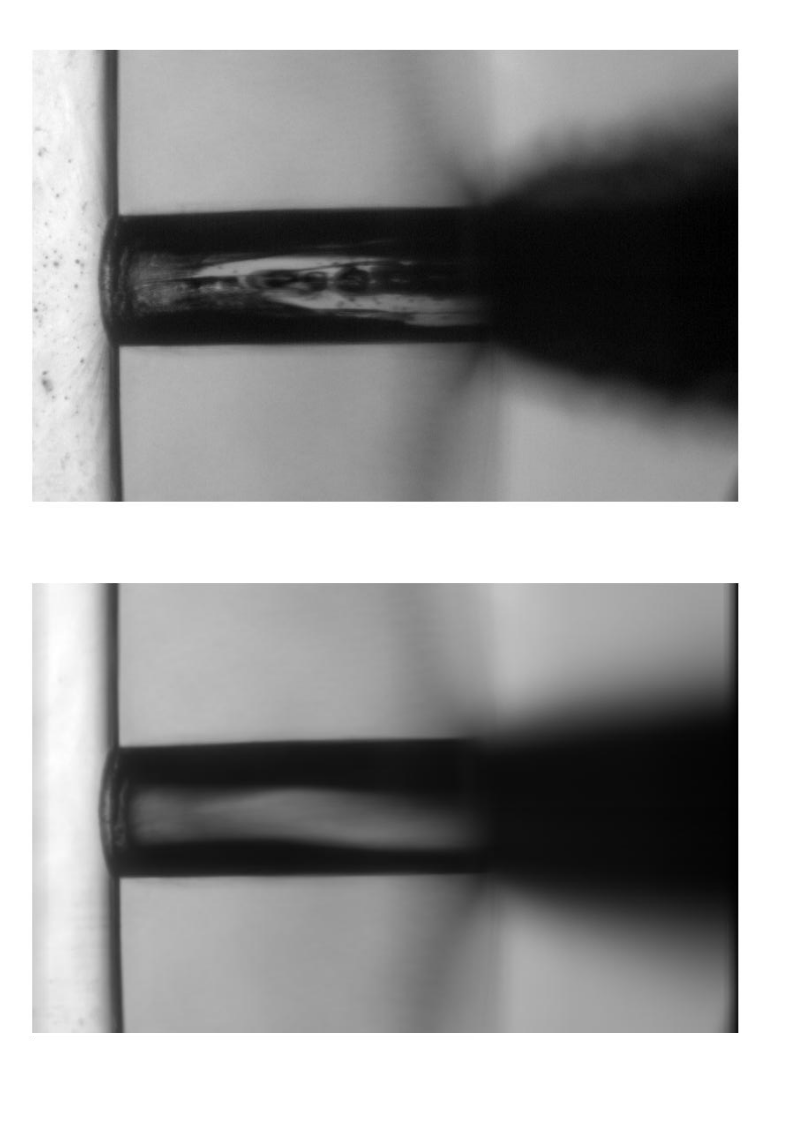
\includegraphics[width=3in]{Zeichnung.png}};
\draw (1.45in,-1.7in) node[]{b)};
\draw (1.45in,0.3in) node[]{a)};
\end{tikzpicture}
\end{center}
\vspace*{-10mm}
\caption{Cavitation in orifice at 50 MPa rail pressure and atmospheric back pressure
         ($CN \approx 390$): a) single shot image with transient, turbulent cavitation
				 phenomena in the orifice center, b) averaged image.}
\label{fig4} 
\end{figure}


The spray that emerges the orifice of the transparent nozzle is unfocused in the shadow images
due to the shallow depth of field of the imaging optics. The dark vertical line on the left side of the image indicates the sac hole wall.
This line is visible since the refractive index of the diesel fuel and the PMMA are
similar but not identical.


\begin{figure}[h]
\begin{center}
\begin{tikzpicture}
\node[inner sep=0pt] (russell) at (0,0){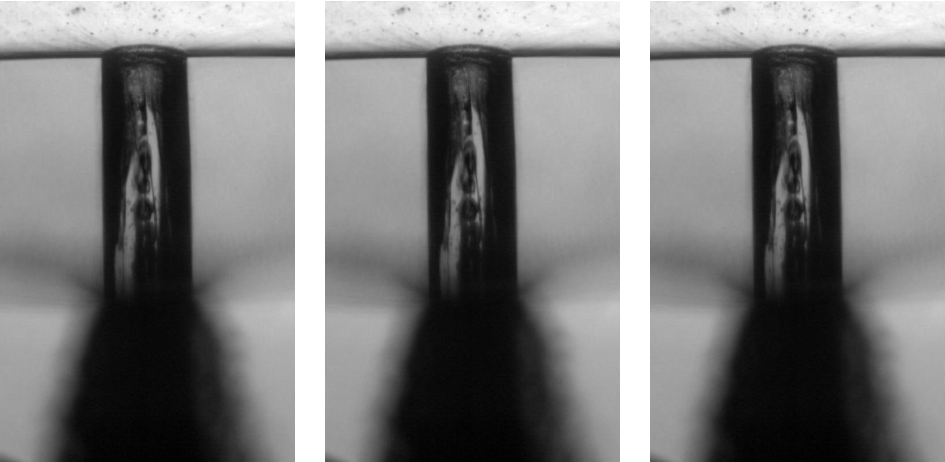
\includegraphics[width=3in]{3_Bild_test}};
\end{tikzpicture}
\end{center}
\vspace*{-2mm}
\caption{Cavitation in orifice at 50 MPa rail pressure and different back pressures of
         1~atm (left), 1.5~MPa (middle) and 3~MPa (right). Note that the images are
				 rotated clockwise by 90$^{\circ}$ compared to figure \ref{fig3} and \ref{fig4}.}
\label{fig5} 
\end{figure}


The cavitation pockets along the orifice walls are visible over the entire length,
which may indicate the occurrence of non-symmetric hydraulic flip.
However, the cavitation is highly unsymmetrical as clearly visible in the averaged image shown
in figure \ref{fig4} b). The cavitation pocket on the top side of the orifice is larger which
can makes sense given the flow direction coming from the top of the sac bore.
%

To eliminate the transient turbulence phenomena in the orifice, the single images
acquired during the steady-state injection process have been averaged over multiple injections. An averaged image is depicted in figure \ref{fig4} b).
%

The transient cavitation phenomena that are visible between the cavitation pockets along the
orifice walls are highly fluctual and different from image to image.  As the images are only
acquired with 20,000~fps the timing between single events is 50~$\mu$s which is too long at
the given velocities to connect the transient events together for further evaluation
(e.g. velocity information).\\
%
Figure \ref{fig5} shows the averaged in-nozzle flow with identical rail pressure (50~MPa)
for different back pressures: 1~atm ($CN \approx 390$), 1.5~MPa ($CN \approx 25$) and 3~MPa
($CN \approx 12$)). The images are rotated clockwise by 90$^{\circ}$ compared to figure
\ref{fig3} and \ref{fig4}. The flow enters the nozzle from the right side and leaves the
orifice to the bottom. The cavitation pocket sizes get smaller with increasing back pressure
(decreasing $CN$) but remain filling the whole length of the orifice on both sides.
%

The in-nozzle flow depicted in figure \ref{fig6} is an averaged image from injections at
80~MPa rail and 3~MPa back pressure ($CN \approx 21$). This pressure ratio represents the
same fuel pressure and air density as in large two-stroke marine diesel engines.
%


\begin{figure}[h]
\begin{center}
\begin{tikzpicture}
\node[inner sep=0pt] (russell) at (0,0){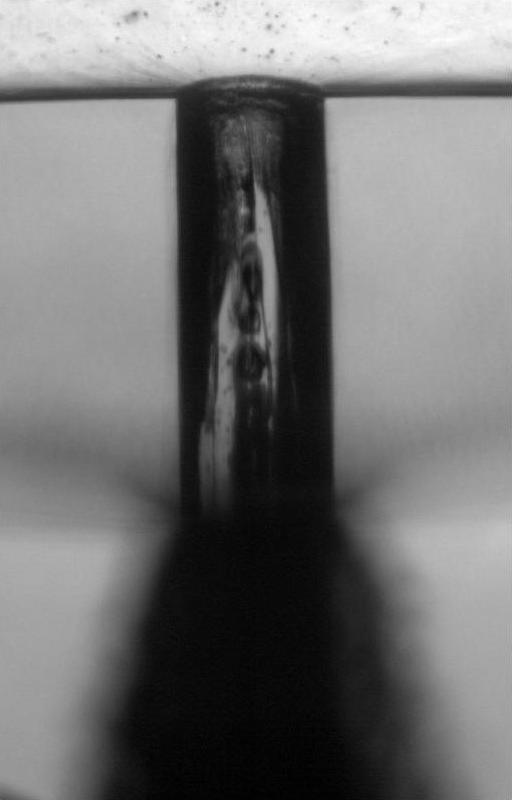
\includegraphics[angle=90, width=3in]{20170227_02_0165_edit}};
\end{tikzpicture}
\end{center}
\vspace*{-2mm}
\caption{Cavitation in orifice at 80 MPa rail pressure and 3~MPa back pressures ($CN \approx 21$).}
\label{fig6} 
\end{figure}


Similar to the images shown from lower injection pressure (see figure \ref{fig4} and \ref{fig5}),
the cavitation emerges over the whole length of the orifice as well.\\
%
The cavitation number for the shown cases at 50~MPa (1.5~MPa back pressure) and 80~MPa
(3~MPa back pressure) rail pressure are similar ($CN \approx 25$ and $CN \approx 21$,
respectively) but the cavitation pockets within the orifice look different when compared
to each other.\\


%CONCLUSIONS
\section*{Conclusions}
The newly developed spray chamber proofs to be a valuable addition to the experimental equipment
at Chalmers. The flushing procedure helps reduce fuel deposits on the windows significantly.
The transparent nozzle holder developed by \cite{Falgout2015} was able to withstand the desired
fuel pressures of up to 80~MPa and the large orifice diameter of 0.75~mm. However, due to space
limitations of the current design, a new transparent nozzle holder has to be developed.
Especially for angled orifices and multi-hole nozzles, the current design is not feasible due
to geometrical restrictions. Additionally, to investigate the transient in-nozzle flow at the
start of injection when the needle in the injector is moving, the design has to be altered to
fit to the non-sac Win~G\&D injectors.\\
%
The qualitative, averaged, quasi-steady state cavitation images can be reproduced with different
PMMA nozzles from the same manufacturing batch. It can therefore be assumed that the
manufacturing tolerances play an unimportant role for the used design.\\
%
The acquired images show small bubbles in the sac bore. Experiments show that the temperature
and the amount of dissolved gas in the fuel change the cavitation pocket size
\cite{Watanabe2014}.
It has therefore to be investigated how the amount of dissolved gas in the diesel used and
the fuel properties itself alters the cavitation properties. It also has to be investigated
how the fuel temperature changes the in-nozzle flow regarding cavitation. This could be realized
by tempering the Win~G\&D injector to different temperatures (in temperature ranges where the
durability of the used thermoplast PMMA is still guaranteed).\\
%
The strongly developed cavitation flow as depicted in the images can be attributed to the
sharp edge design of the nozzle. As this sharp edge between sac bore and orifice is not
realistic for commercial injectors (as usually radii are machined by either electrochemical
machining or hydro-erosive grinding), nozzle geometry variations (inlet radius, taper and angle)
will be investigated in future work.\\
%
Additionally, simultaneous optical measurements of in-nozzle flow and primary spray breakup
will be the next step in this project as well as first CFD validation within the simulation
groups at Win~G\&D and Combustion Division at Chalmers.\\
%



%ACKNOWLEDGMENT
\section*{Acknowledgment}
The authors would like to thank the Combustion Engine Research Center (CERC),
the Swedish Energy Agency and the Swiss Federal Office of Energy for funding.
Special thanks to Mark~Linne and Zachary Falgout for their support.
\newline

%REFERENCES
\bibliography{ilass}
\bibliographystyle{ilass}

\end{document}
\end

